% Created 2014-11-03 Mon 16:13
\documentclass[9pt,b5paper]{article}
\usepackage{graphicx}
\usepackage{xcolor}
\usepackage{xeCJK}
\usepackage{longtable}
\usepackage{float}
\usepackage{textcomp}
\usepackage{geometry}
\geometry{left=0cm,right=0cm,top=0cm,bottom=0cm}
\usepackage{multirow}
\usepackage{multicol}
\usepackage{listings}
\usepackage{algorithm}
\usepackage{algorithmic}
\usepackage{latexsym}
\usepackage{natbib}
\usepackage{fancyhdr}
\usepackage[xetex,colorlinks=true,CJKbookmarks=true,linkcolor=blue,urlcolor=blue,menucolor=blue]{hyperref}


\lstset{language=c++,numbers=left,numberstyle=\tiny,basicstyle=\ttfamily\small,tabsize=4,frame=none,escapeinside=``,extendedchars=false,keywordstyle=\color{blue!70},commentstyle=\color{red!55!green!55!blue!55!},rulesepcolor=\color{red!20!green!20!blue!20!}}
\author{Jenny Huang}
\date{\today}
\title{Android App Programming Directed Study \textasciitilde{} DrawingFun}
\hypersetup{
  pdfkeywords={},
  pdfsubject={},
  pdfcreator={Emacs 24.3.1 (Org mode 8.2.7c)}}
\begin{document}

\maketitle
\tableofcontents


\section{first checkin 10/27/2014}
\label{sec-1}
\subsection{Goal}
\label{sec-1-1}
\begin{itemize}
\item According to the instructor's requirements that we are going to implement an simple window's Paint like Android app for later on integrating Union’s 2D graphics to Android app.
\end{itemize}
\subsection{Course Introduction}
\label{sec-1-2}
\begin{itemize}
\item We have only two students, the other one is an undergraduate exchange students with solid Java programming background and relatively slightly week problem-solving skills. For the first more than half semester, we used Sudoku as the starting point and tried several different topics to get our hands wet.
\end{itemize}
\subsection{Project Introduction}
\label{sec-1-3}
\begin{itemize}
\item It's after middle term already, the way we were currently trying on to make it work may just work perfectly for the other classmate, but for me, I feel like it takes forever for me to be able to make any significant progress. So about half a month ago, I was motivated and thought instead of surfacing around and having fun learning by trial and error, maybe I should start from an simple GUI app as a starting point and try my best to expend/extend the APP functionality from there. And also we would be able to work to our final project slightly earlier.
\item This GUI will be my very second GUI interface that I have ever created for my Computer Science major, (this first one was an Python Tkinter GUI one week short project for plotting graphics with data abstracted from back end database during an intern-ship;). And I guess it may still be slightly difficult for me to start write Android App code of my own line by line, so I simply searched internet, and trying an tutorial to make a working starting point Android Paint GUI. I integrated the codes from the reference link all together, fixed minor compile errors, and it worked!
\item This "Copied" GUI will serve as the starting point, and my functionality updates start from here, and I will update my progress for this project later on by week according to the instructor's requirements and suggestions.
\end{itemize}
\subsection{References}
\label{sec-1-4}
\begin{itemize}
\item \url{http://code.tutsplus.com/tutorials/android-sdk-create-a-drawing-app-interface-creation--mobile-19021}
\end{itemize}
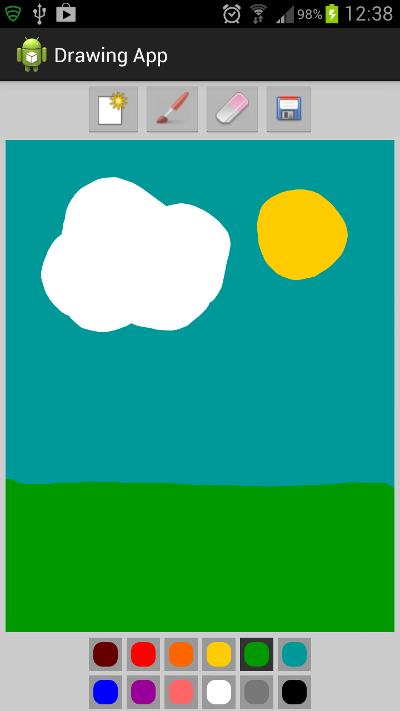
\includegraphics[width=.6\linewidth]{./android_drawing_final.png}

\section{Checkin for 11/3/2014}
\label{sec-2}
\subsection{Buttons I have worked on}
\label{sec-2-1}
\subsubsection{Color\textunderscore Picker:}
\label{sec-2-1-1}
\subsubsection{Undo/Redo:}
\label{sec-2-1-2}

\subsection{Functionalities and References}
\label{sec-2-2}
\subsubsection{Color\textunderscore Picker:}
\label{sec-2-2-1}
\begin{itemize}
\item Motivated by the Picasso Android app, seeing their multiple color choices, our starting point \textbf{12} fixed colors were too limited.
\end{itemize}
\subsubsection{Undo/Redo Buttons:}
\label{sec-2-2-2}
\begin{itemize}
\item Also motivated by the Picasso app, intended to work on \textbf{Undo} button, and ended up found \textbf{Redo} button could be very convenient as well.
\item needs to update these Undo/Redo methods later on, this is just the starting point most basic implementation for this button set.
\end{itemize}
\subsubsection{Snapshot}
\label{sec-2-2-3}
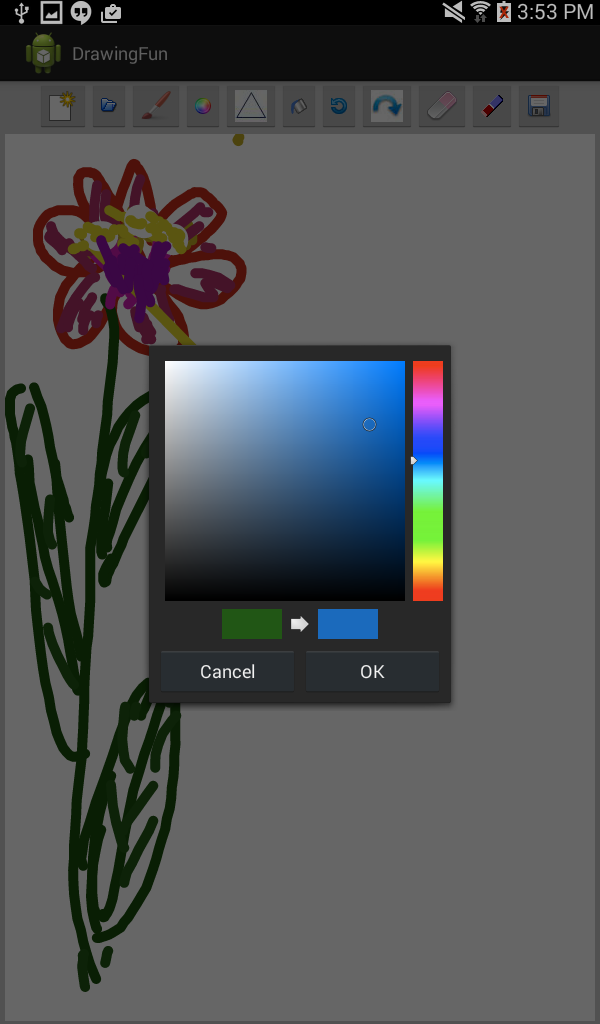
\includegraphics[width=.6\linewidth]{./20141103.png}

\subsection{Todo}
\label{sec-2-3}
\subsubsection{Load image file button}
\label{sec-2-3-1}
\subsubsection{Drawing shapes with Finger for primitives}
\label{sec-2-3-2}
refer to the reference below: 
\begin{itemize}
\item \url{http://gmariotti.blogspot.com/2014/01/drawing-shapes-with-fingers.html}
\end{itemize}
\subsubsection{Erase Rectangle}
\label{sec-2-3-3}
\subsubsection{Undo/Redo}
\label{sec-2-3-4}
% Emacs 24.3.1 (Org mode 8.2.7c)
\end{document}